%\pgfdeclarelayer{background}
%\pgfdeclarelayer{foreground}
%\pgfsetlayers{background,main,foreground}

\pgfplotsset{
	axis background/.style={fill=none},
	%tick style=mygrey2,
	%tick label style=mygrey2,
	grid=none,
	legend style={font=\small},
	%xtick pos=left,
	%ytick pos=left,
	tick style={
		major grid style={style=white,line width=1pt},minor grid style=white,
		%		major grid style={style=white,line width=1pt},minor grid style=mygrey3,
		%tick align=outside,
	},
	%minor tick num=4,
}

\begin{figure}[tb]
	\centering
	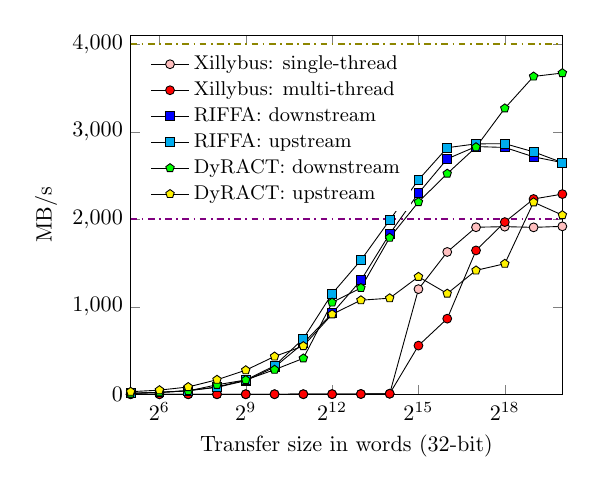
\begin{tikzpicture}[scale = 0.8]
	\begin{axis}[
	xmode=log,
	log basis x={2},
	xlabel=Transfer size in words (32-bit),
	ymin=0,
	ymax=4100,
	xmax = 1048576,
	xmin = 32,
	ylabel=MB/s,
	%	 legend style={at={(0.3,0.8)},anchor=north}
	legend cell align={left},
	legend pos=north west,
	legend style={draw=none}
	]    
	
	\addplot [mark=*,mark options={fill=pink}] plot coordinates {
		(32,     0)
		(64,     0)
		(128,    0.05)
		(256,     0.1)
		(512,      0.2)
		(1024,     0.35)
		(2048,     0.7)
		(4096,     1.45)
		(8192,     2.9)
		(16384,    5.85)
		(32768,    1201.5)
		(65536,    1626.5)
		(131072,   1909.1)
		(262144,   1915.8)
		(524288,   1907.7)
		(1048576,  1919.1)	
	}; 
	\addplot [mark=*,mark options={fill=red}] plot coordinates {
		(32,     0)
		(64,     0)
		(128,    0.04)
		(256,    0.08)
		(512,    0.16)
		(1024,   0.32)
		(2048,   0.68)
		(4096,   1.36)
		(8192,   2.76)
		(16384,  5.85)
		(32768,  556)
		(65536,  864)
		(131072, 1644)
		(262144, 1968)
		(524288, 2232)
		(1048576, 2288)
	}; 
	
	\addplot [mark=square*,mark options={fill=blue}] plot coordinates {
		(32,     11.1)
		(64,     20.3)
		(128,    41.0)
		(256,    78.8)
		(512,    155.0)
		(1024,   310.0)
		(2048,   583.0)
		(4096,   924.6)
		(8192,   1302.1)
		(16384,  1832.8)
		(32768,  2297.8)
		(65536,  2691.1)
		(131072, 2831.3)
		(262144, 2821.2)
		(524288, 2713.9)
		(1048576,2647.7)	
	}; 
	\addplot [mark=square*,mark options={fill=cyan}] plot coordinates {
		(32,     11.1)
		(64,     21.0)
		(128,    41.4)
		(256,    83.5)
		(512,    162.8)
		(1024,   325.5)
		(2048,   635.2)
		(4096,   1148.9)
		(8192,   1531.9)
		(16384,  1990.4)
		(32768,  2451.0)
		(65536,  2818.5)
		(131072, 2862.0)
		(262144, 2864.5)
		(524288, 2771.1)
		(1048576,2647.7)
	}; 
	
	\addplot [mark=pentagon*,mark options={fill=green}] plot coordinates {
		(32,     7.7)
		(64,     22.2)
		(128,    37.7)
		(256,    108.1)
		(512,    163.2)
		(1024,   280.7)
		(2048,   410.2)
		(4096,   1049.2)
		(8192,   1215.4)
		(16384,  1790.2)
		(32768,  2197.4)
		(65536,  2522.2)
		(131072, 2824.7)
		(262144, 3268.9)
		(524288, 3633.0)
		(1048576,3671.9)	
	}; 
	\addplot [mark=pentagon*,mark options={fill=yellow}] plot coordinates {
		(32,     29)
		(64,     47)
		(128,    83)
		(256,    166)
		(512,    275)
		(1024,   432)
		(2048,   551)
		(4096,   914)
		(8192,   1075)
		(16384,  1098)
		(32768,  1343)
		(65536,  1151)
		(131072, 1416)
		(262144, 1492)
		(524288, 2195)
		(1048576,2048)
	}; 
	
	\addplot [color=violet,thick,dash dot] plot coordinates {
		(32,     2000)
		(64,     2000)
		(128,     2000)
		(256,     2000)
		(512,     2000)
		(1024,     2000)
		(2048,     2000)
		(4096,     2000)
		(8192,     2000)
		(16384,    2000)
		(32768,    2000)
		(65536,    2000)
		(131072,    2000)
		(262144,    2000)
		(524288,    2000)
		(1048576,   2000)	
	};
	
	\addplot [color=olive,thick,dash dot] plot coordinates {
		(32,     4000)
		(64,     4000)
		(128,     4000)
		(256,     4000)
		(512,     4000)
		(1024,     4000)
		(2048,     4000)
		(4096,     4000)
		(8192,     4000)
		(16384,    4000)
		(32768,    4000)
		(65536,    4000)
		(131072,   4000)
		(262144,   4000)
		(524288,   4000)
		(1048576,  4000)	
	};
	
	\legend{Xillybus: single-thread\\Xillybus: multi-thread\\RIFFA: downstream\\RIFFA: upstream\\DyRACT: downstream\\DyRACT: upstream\\}
	\end{axis}
	\end{tikzpicture} 
	%	\label{riffa_loopback_bw}
	%	}
	
	\caption[]{PCIe system loopback test evaluation.} 
	\label{pcie_xillybus_riffa_loopback_bw}
	
\end{figure}
